\section{Experiment 9G: finite-data personalized federated identification}
\label{sec:experiment9g}

\paragraph{Question and protocol.}
Experiment 9F establishes that oracle client coordinates on a shared manifold
can preserve individual control performance. Experiment 9G removes that oracle:
can shared backbones be learned from client messages and can an unseen client
identify only its local coordinate from finite records?

For each of ten fresh seeds (166--175), 180 training clients apply the frozen
9D adaptive acquisition policy. They transmit their three-dimensional
structured estimate and normalized covariance, not raw trajectories. The server
selects an unknown number of groups with the heteroscedastic mixture from
Experiment 9D and learns a control-aware center and rank-one or rank-two basis
from the estimates assigned to each group. This is a one-shot federated-summary
protocol rather than iterative gradient FL; privacy is not applied in 9G.

Each of 30 unseen clients begins with the same three 0.25~s records and one
one-second complementary record, for 1.75~s total. For every candidate group it
fits only $a_i\in\mathbb{R}^r$ on the three initial records. It selects the group
with the lowest error on the held-out complementary record, then refits only
that group's $r$ coefficients on all records. No true test parameter is used.
Learned-rank methods use the unknown-$K$ groups; Oracle-group variants replace
only the training grouping by true simulator families. Local fits all three
ratios from the same records, and Exact-individual remains an unattainable
reference.

The rank-one gate requires Learned-rank-1 to lie within 2\% of Local. The
rank-two gate is stricter: Learned-rank-2 must be no worse than Local. These
criteria were fixed before inspecting the fresh seeds.

\begin{table}[htbp]
\centering
\caption{Experiment 9G finite-data tracking on ten fresh fleets.}
\label{tab:experiment9g-results}
\begin{tabular}{lrrrr}
\toprule
Method & Groups & Local dim. & Tracking & vs. Local\\
\midrule
Exact-individual & --- & 3 & 0.006679 & $-4.25\%$\\
Local & --- & 3 & 0.006975 & ---\\
Learned rank 1 & 3.0 & 1 & 0.007474 & $+7.16\%$\\
Learned rank 2 & 3.0 & 2 & 0.007018 & $+0.61\%$\\
Oracle-group rank 1 & 3 & 1 & 0.007512 & $+7.70\%$\\
Oracle-group rank 2 & 3 & 2 & 0.007018 & $+0.62\%$\\
\bottomrule
\end{tabular}
\end{table}

\begin{figure}[htbp]
\centering
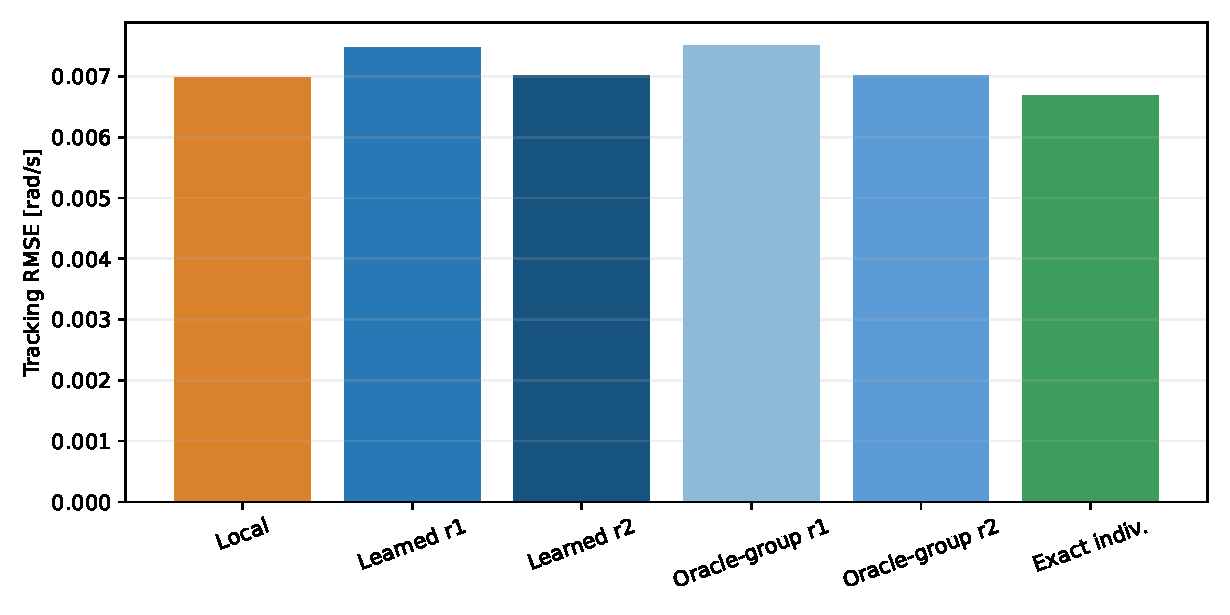
\includegraphics[width=0.82\linewidth]{../results/figures/experiment_9g_finite_personalized.pdf}
\caption{Finite-data personalized models compared with full Local and the exact
individual reference.}
\label{fig:experiment9g}
\end{figure}

\paragraph{Results.}
The server selects three groups in every fleet and reaches mean training ARI
0.951. Learned-rank-2 is only 0.61\% worse than Local on average and wins four
of ten paired fleets; its fleet-wise relative difference ranges from $-1.25\%$
to $+2.57\%$. Its scheduled-gain error is 0.00577, essentially the same as
Local's 0.00578, even though its unweighted parameter error is larger (0.0745
versus 0.0699). This is practically near-parity with one fewer locally estimated
coordinate, but it fails the predeclared requirement of being no worse than
Local.

Rank one does not preserve its oracle promise. Learned-rank-1 is 7.16\% worse
than Local, exceeds the 2\% tolerance, and wins only one fleet. The corresponding
Oracle-group result is 7.70\% worse. For rank two, Learned and Oracle-group
tracking differ by less than 0.01 percentage points relative to Local. Hence the
remaining loss is not caused by unknown group discovery. It arises because
finite short-data estimation of the manifold coordinates and backbones does not
realize the oracle projections used in 9F.

All 2100 adaptive client fits and all personalized coefficient fits converge.
All 5400 nonlinear closed-loop evaluations remain feasible. Both formal gates
fail, so 9G supports a compression--performance tradeoff, not a claim that
personalized federation improves absolute tracking.

\paragraph{Interpretation and decision.}
The result materially changes the FL conclusion. A personalized formulation is
reasonable: rank two reproduces Local gain quality and nearly reproduces its
tracking while transferring a shared group backbone. However, with only three
original parameters, reducing the local head from three coordinates to two is a
modest compression. It is not by itself a sufficiently strong headline unless
the two-coordinate estimator can also demonstrate less calibration, improved
uncertainty, privacy benefits, or better adaptation for new clients.

Further algorithmic work should target the actual bottleneck exposed here rather
than clustering. Candidate improvements are joint uncertainty-aware estimation
of backbone and coefficients, direct control-loss validation of $a_i$, and
adaptive acquisition targeted along the missing manifold direction. A particularly
clean next test would compare how much data Local and rank two require to reach a
fixed tracking or gain-error tolerance. If rank two reaches Local-quality control
with materially less excitation, personalized FL gains an operational purpose.
If it needs the same data, the current three-parameter benchmark is probably too
small to sustain a strong personalized-FL contribution on compression alone.

\paragraph{Reproducibility.}
The frozen configuration is \path{code/config/experiment_9g.json}; the implementation
is \path{code/experiments/experiment_9g_finite_personalized.py}. Aggregate and
seed-level results, group diagnostics, assignments, comparisons, and provenance
hashes are stored under \path{results/tables}.
